\chapter{Práctica: Aspiradora autónoma (con autolocalización)}\label{cap.roomba}
En este capítulo se expondrá el desarrollo de una nueva práctica para la plataforma de JdeRobot-Academy, denominada ``Aspiradora autónoma (con autolocalización)''. Se aborda el desarrollo de su infraestructura, su componente académico correspondiente, así como el evaluador automático creado y la solución de referencia llevada a cabo. 


\section{Enunciado} \label{sec.enunciado}
En esta nueva práctica, el objetivo principal es lograr que un robot aspirador autónomo consiga barrer la mayor superficie posible de un apartamento. Para ello deberá hacer uso de su capacidad de autolocalización y del mapa de dicho apartamento. Esta aspiradora además de poseer un sensor de posición que le permite saber su posición y orientación, tiene un actuador de movimiento con el que controla su velocidad lineal y velocidad de giro. Además, posee un sensor láser que le permite medir la distancia a la que se sitúan los obstáculos y un sensor de choque que no serán utilizados en el desarrollo de la solución de referencia. \\

En esta práctica el alumno deberá programar un algoritmo capaz de recorrer un gran porcentaje de la casa usando la capacidad de autolocalización del robot que deberá ofrecer la planificación de una ruta en forma de zigzag. Después, deberá proporcionar un algoritmo de pilotaje para que la aspiradora siga dicha ruta. En la interfaz gráfica creada se puede observar el mapa de la casa, así como la posición de la aspiradora en dicho mapa y la superficie recorrida. Este mapa estará disponible para realizar el algoritmo de control y también se usará para la medida de la nota final.


\section{Infraestructura} 
En este apartado se describirá el entorno que se ha creado para poder realizar la práctica ``Aspiradora autónoma (con autolocalización)''. Primero se describirá el modelo del robot aspirador utilizado, incluyendo sus sensores y actuadores. Después, se explicará el mundo simulado (un apartamento típico, con distintas habitaciones y muebles) por el cual se moverá la aspiradora. 

\subsection{Modelo Roomba}
El modelo del robot aspirador encargado de ejecutar el algoritmo programado está basado en los robots Roomba de la empresa iRobot. Inicialmente, este modelo se diseñó para realizar un algoritmo de navegación sin autolocalización por lo que está inspirado en el Roomba de la serie 500 (ver Figura~\ref{fig.roomba500}). 

\begin{figure}[H]
  \begin{center}
    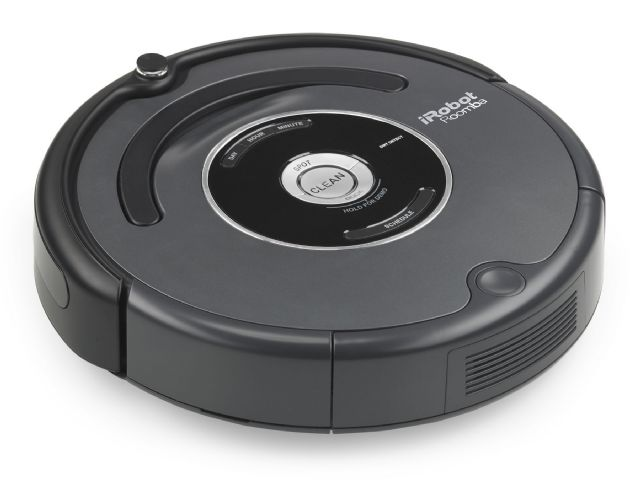
\includegraphics[width=0.4\textwidth]{figures/Vacuum/roomba500.jpg}
		\caption{Roomba 500 de iRobot}
		\label{fig.roomba500}
		\end{center}
\end{figure}

El modelo Roomba de JdeRobot tiene instalados un sensor láser y un sensor de choque que no serán necesarios para la realización de la solución de esta práctica. Además, posee un sensor de posición que se utilizará para obtener tanto la orientación del robot como sus coordenadas en el sistema de referencia del simulador Gazebo. También dispone de un actuador de movimiento que permite que se desplace por el mundo de Gazebo. \\

En esta práctica se han empleado los siguientes \textit{plugins} para este modelo:

\begin{itemize}
\item pose3di: Este \textit{plugin} se emplea para obtener las coordenadas del robot en tiempo real y su orientación.
\item motorsi: Este \textit{plugin} interactúa con el componente permitiendo dotar al robot de velocidad lineal y velocidad de giro.
\end{itemize}

En la Figura~\ref{fig.vacuumModel} se puede observar el modelo \textit{Roomba} de JdeRobot que mide aproximadamente 330 mm de ancho, 90 mm de altura, y un peso de 2.5 kg.\\

\begin{figure}[H]
  \begin{center}
    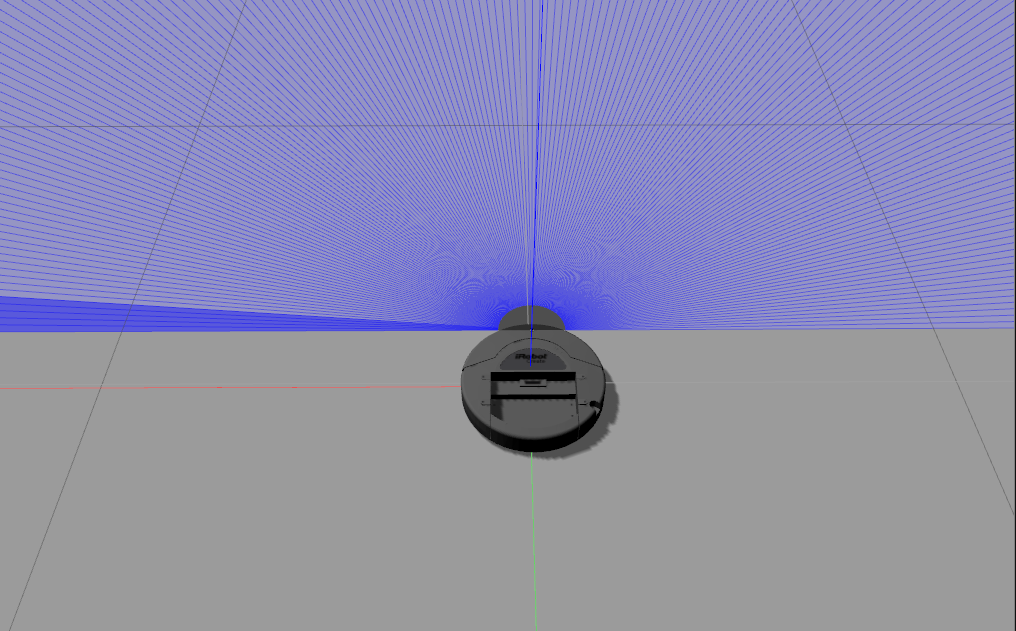
\includegraphics[width=0.7\textwidth]{figures/Vacuum/vacuumModel.png}
		\caption{Modelo Roomba}
		\label{fig.vacuumModel}
		\end{center}
\end{figure}


\subsection{Modelo house\_int2}
Ha sido necesario crear el modelo de un apartamento para que la aspiradora pueda navegar por ella. El modelo está basado en el modelo de casa que empleó Juan Navarro en su proyecto Fin de Carrera~\cite{localization1} en el mundo \textit{GrannyAnnie.world} (Figura~\ref{fig.GrannyAnnie}).\\

\begin{figure}[H]
  \begin{center}
    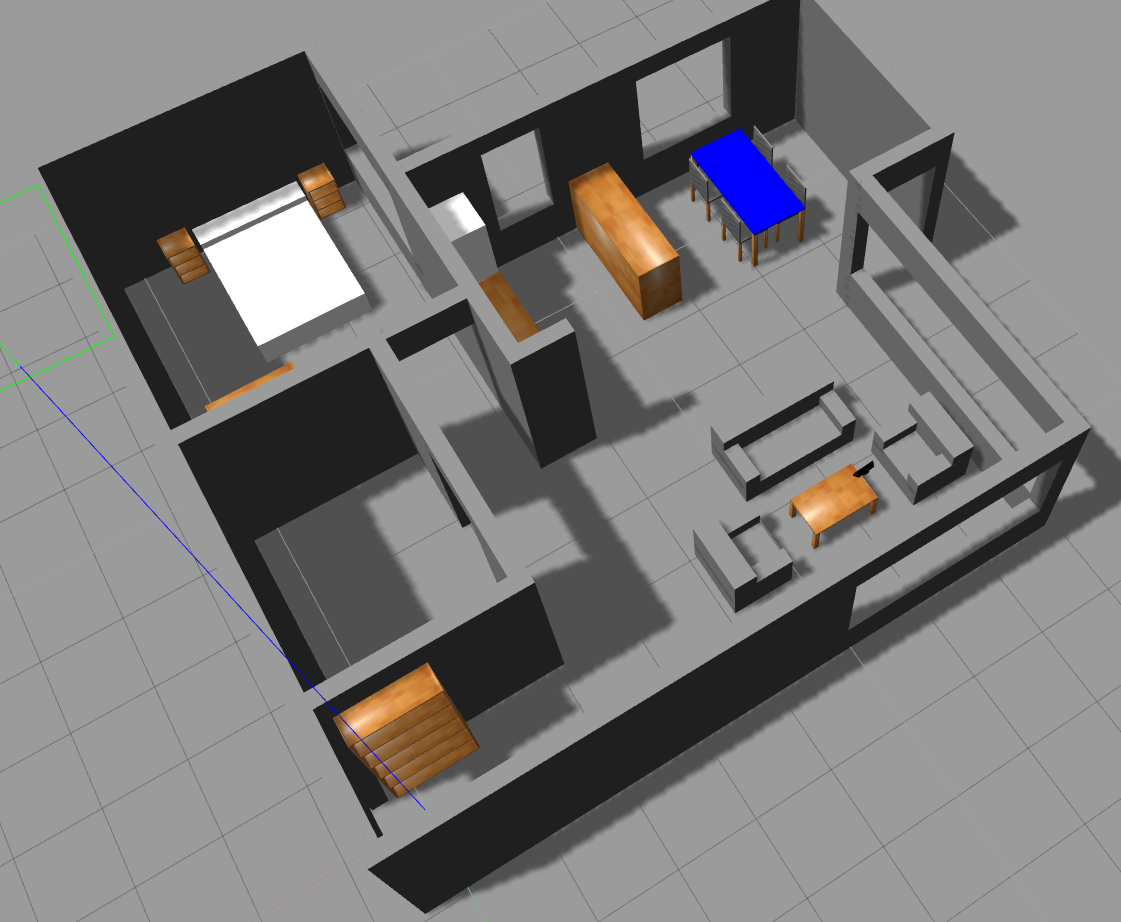
\includegraphics[width=1.0\textwidth]{figures/Vacuum/GrannyAnnie.png}
		\caption{Mundo GrannyAnnie.world}
		\label{fig.GrannyAnnie}
		\end{center}
\end{figure}

Inicialmente, este modelo se utilizó para un problema de navegación sin autolocalización por lo que fue necesario realizar algunas modificaciones. Debido a que el pilotaje de la aspiradora se basaba en un algoritmo de ``choca-gira'', cabía la posibilidad de que la aspiradora se saliese de la casa por lo que se eliminaron las puertas exteriores la misma. También, se modificó la malla de colisiones de algunas paredes ya que la aspiradora podía atravesarlas. Por último, se aumentó la masa del inmobiliario de la casa ya que la masa que tenían inicialmente no era suficiente por lo que la aspiradora al chcocar con los muebles los desplazaba. El nuevo modelo de casa se llama \textit{``house\_int2''} y se puede ver ver en la Figura~\ref{fig.house_int2}, donde aparecen los cambios marcados en rojo.\\


\begin{figure}[H]
  \begin{center}
    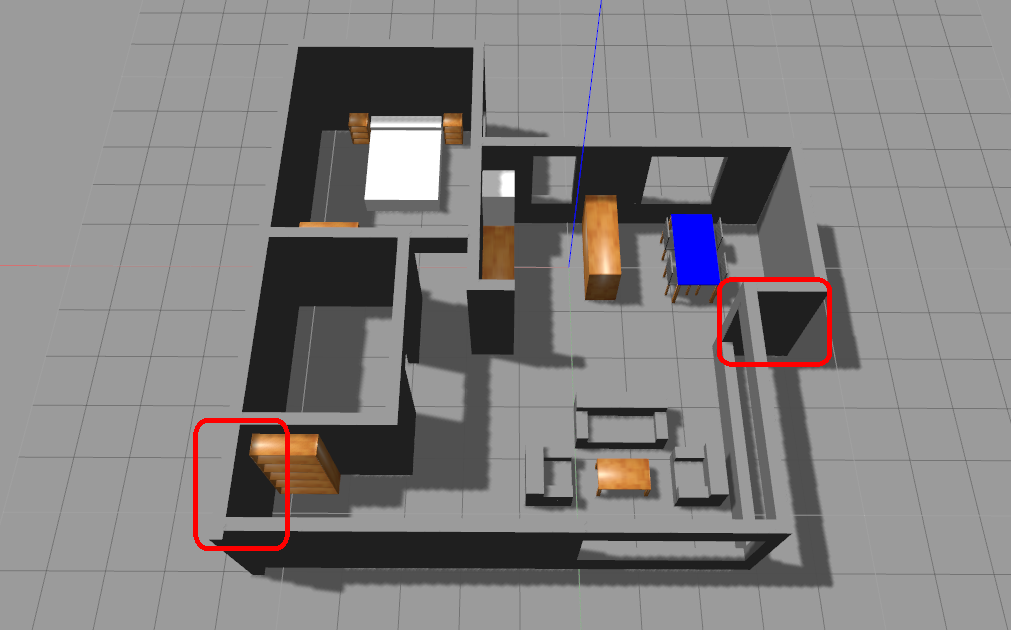
\includegraphics[width=1.0\textwidth]{figures/Vacuum/house_int2.png}
		\caption{Modelo house\_int2}
		\label{fig.house_int2}
		\end{center}
\end{figure}



\subsection{Mundo de Gazebo}
Para esta práctica se ha creado un mundo 3D en Gazebo formado por el modelo de la casa \textit{``house\_int2''} y por el robot aspirador \textit{``Roomba''}, que ejecutará la solución desarrollada. También se ha añadido una fuente de luz mediante la etiqueta \texttt{<light>}.\\

Para tener este escenario se ha creado el siguiente mundo en Gazebo llamado \textit{``vacuum.world''}:

\vspace{20pt}
	\begin{lstlisting}[frame=single]
<?xml version="1.0" ?>
<sdf version='1.4'>
	<world name='Vacuum'>
    	<include>
    	     <uri>model://roomba</uri>
    	     <pose>5.04 3.80 0 0 0 -1.57 </pose>
    	  	 <!--<pose>5.04 3.80 0 0 0 -1.57 </pose> Room-->
    	  	 <!--<pose>5.04 0.00 0 0 0 -1.57 </pose> Bedroom-->
    	  	 <!--<pose>-2.35 5.44 0 0 0 -1.57 </pose> Living room-->
    	  	 <!--<pose>-3.50 1.45 0 0 0 -1.57 </pose> Dining room-->
    	</include>
    	<include>
    	     <uri>model://house_int2</uri>
    	  	 <pose>0 0 0 0 0 0</pose>
    	</include>
		<include>
    	     <uri>model://ground_plane_transparent</uri>
    	</include>
    	
    	<light name='sun' type='directional'>
      		<cast_shadows>1</cast_shadows>
      		<pose>0 0 10 0 -0 0</pose>
      		<diffuse>0.8 0.8 0.8 1</diffuse>
      		<specular>0.2 0.2 0.2 1</specular>
      		<attenuation>
        		<range>1000</range>
        		<constant>0.9</constant>
        		<linear>0.01</linear>
        		<quadratic>0.001</quadratic>
      		</attenuation>
      		<direction>-0.5 0.1 -0.9</direction>
    	</light>
    
		<scene>
		  	<ambient>0.4 0.4 0.4 1</ambient>
		  	<background>0.7 0.7 0.7 1</background>
		  	<shadows>1</shadows>
		</scene>
    
		<gui fullscreen='0'>
		  <camera name='user_camera'>
		    <pose>0.126197 6.13852 18.8314 0 1.08764 -2.14299</pose>
		    <view_controller>orbit</view_controller>
		  </camera>
		</gui>
  </world>
</sdf>

	\end{lstlisting}


En la Figura~\ref{fig.vacuumWorld} se puede observar el mundo creado en Gazebo.

\begin{figure}[H]
  \begin{center}
    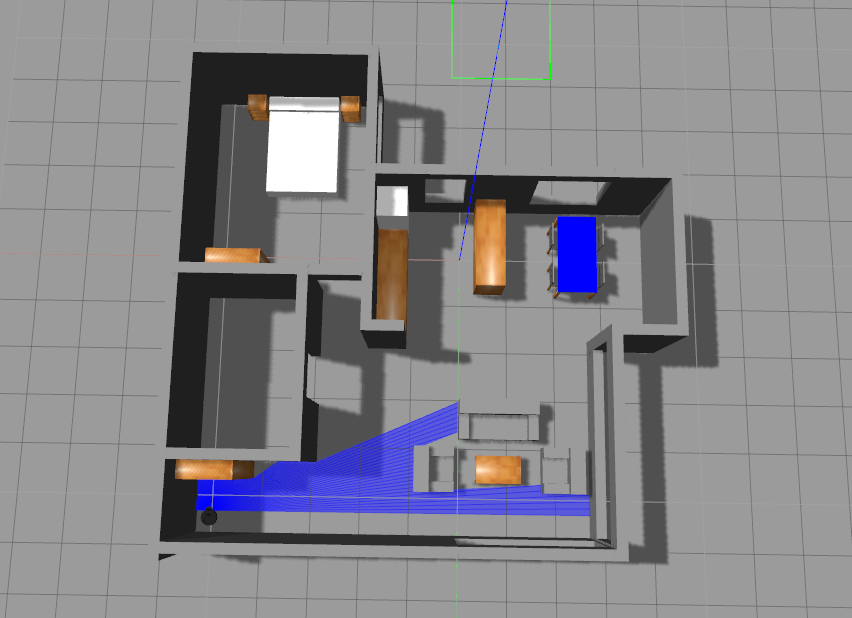
\includegraphics[width=1.0\textwidth]{figures/Vacuum/vacuumWorld.png}
		\caption{Mundo vacuum.world en Gazebo}
		\label{fig.vacuumWorld}
		\end{center}
\end{figure}


\section{Componente académico}
Se ha creado un componente académico para esta práctica que resuelve diversas funcionalidades: (a) muestra una interfaz gráfica al usuario, con distintos elementos, que permiten depurar el código de manera más sencilla; (b) ofrece acceso a sensores y actuadores en forma de métodos simples ocultando el \textit{middleware} de comunicaciones; (c) incluye código auxiliar que ayuda a programar la solución. El componente deja todo listo para que el estudiante sólo tenga que incorporar su código rellenando el método \textit{execute} en el fichero \textit{MyAlgorithm.py}.\\

Este componente ofrece al programador del algoritmo este \acrshort{api} de sensores y actuadores:

\begin{itemize}
\item 	\textit{pose3d.getX()}: Permite obtener la posición absoluta del robot en el eje X.
\item	\textit{pose3d.getY()}: Permite obtener la posición absoluta del robot en el eje Y.
\item	\textit{pose3d.getYaw()}: Permite obtener la orientación del robot con respecto al sistema de referencia de Gazebo.
\item 	\textit{motors.sendV()}: Para establecer la velocidad lineal.
\item	\textit{motors.sendW()}: Para establecer la velocidad de giro.
\end{itemize}

Es necesario crear un archivo de configuración (\textit{vacuum.cfg}) donde se indican los puertos utilizados por los distintos \textit{plugins}, la velocidad lineal máxima y la velocidad angular máxima de los motores.:

\vspace{20pt}
	\begin{lstlisting}[frame=single]
Vacuum.Motors.Proxy = Motors:default -h localhost -p 9003
Vacuum.Pose3D.Proxy = Pose3D:default -h localhost -p 9003
Vacuum.Laser.Proxy  = Laser:default -h localhost -p 9003
Vacuum.Bumper.Proxy  = Bumper:default -h localhost -p 9003
Vacuum.Motors.maxV = 5
Vacuum.Motors.maxW = 20
	\end{lstlisting}

Gracias a la nueva configuración de JdeRobot en su versión actual, se puede usar el mismo puerto para diferentes \textit{plugins}. En esta práctica, se emplea el puerto 9003 para todos los plugins y se ha establecido la velocidad máxima de tracción y de rotación.\\

El componente emplea dos hilos de ejecución, de esta manera se pueden realizar todas las tareas necesarias para el funcionamiento correcto de la práctica. Los hilos utilizados son los siguientes:

\begin{itemize}
\item	Hilo de control: se encarga de actualizar de manera constante los datos captados por los sensores y los datos enviados a los actuadores. Debido a que se trata de una solución reactiva es necesario que el intervalo de actualización de dichos datos sea un tiempo muy corto, en este caso, 50 ms. Si se fijara un tiempo muy grande podría ocasionar errores en la trayectoria del robot.
\item	Hilo de la \acrshort{gui}: este hilo actualiza la interfaz gráfica que se muestra al usuario. Este intervalo de actualización debe de ser también corto ya que la interfaz gráfica es una herramienta que utiliza el programador para depurar su código y debe de mostrar de manera fiable los datos del robot en tiempo real. Este intervalo también es de 50 ms.
\end{itemize}

\subsection{Interfaz gráfica}
La interfaz gráfica de usuario (\acrshort{gui}) de la práctica sirve para representar información importante de ayuda para resolver de manera más sencilla el algoritmo. Además, esta interfaz permite ejecutar el código donde se desarrolla la solución correspondiente. Se ha empleado la herramienta PyQt5 para su desarrollo.\\

En la parte izquierda de la interfaz, se muestra el mapa del apartamento que la aspiradora tiene que recorrer (ver Figura~\ref{fig.mapa}). Es una imagen binaria en la que los obstáculos de la casa (muebles, paredes, etc) aparecen coloreados en negro (valor 0) y la superficie por la que la aspiradora puede pasar libremente aparece en blanco (valor 255). Este mapa se ha realizado manualmente, por lo que si se utilizara otra casa, habría que realizar un nuevo mapa. En este mapa también aparece un triángulo con las aristas en color rojo que indica la posición y la orientación de la aspiradora en tiempo real. Por último, también se marca en color azul, las zonas de la casa por las que la aspiradora ya ha pasado.

\begin{figure}[H]
  \begin{center}
    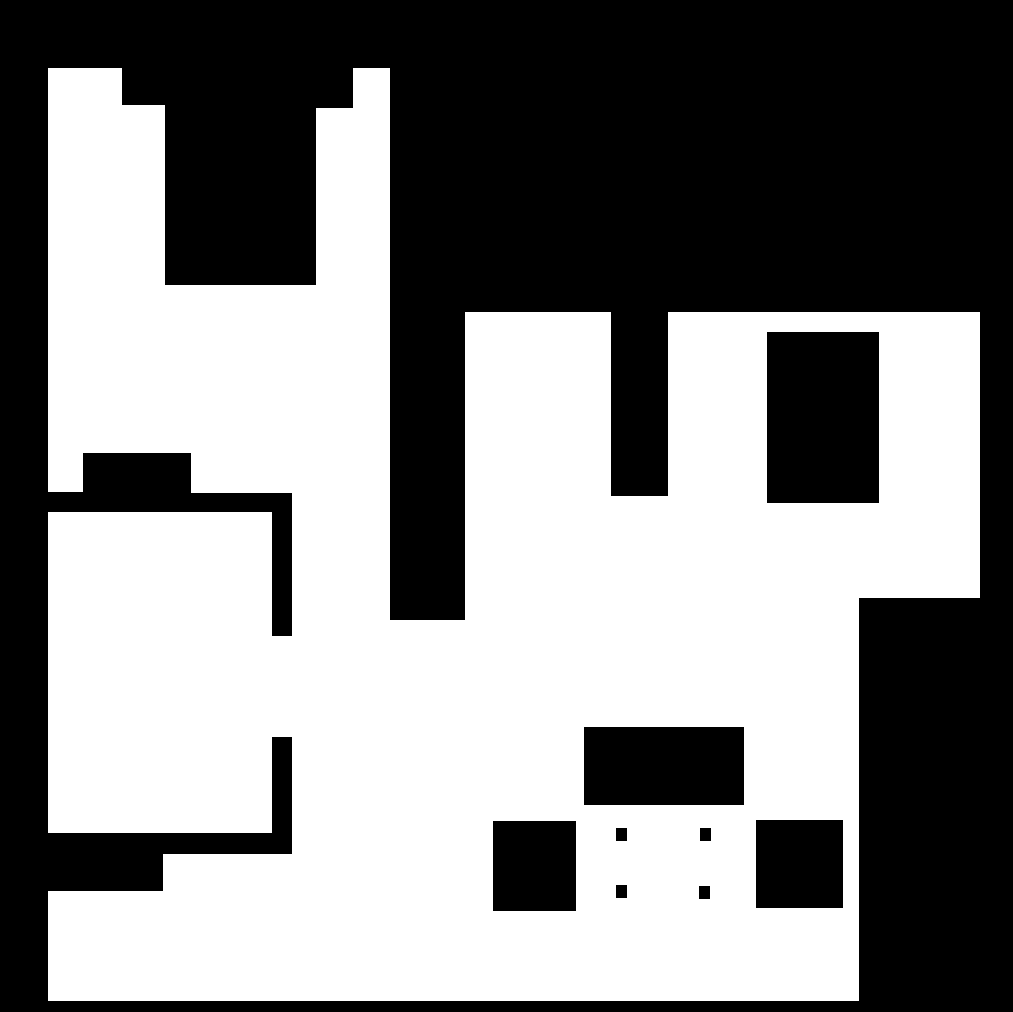
\includegraphics[width=0.7\textwidth]{figures/Vacuum/mapa.png}
		\caption{Mapa de la casa}
		\label{fig.mapa}
		\end{center}
\end{figure}


Tanto como para representar a la aspiradora en el mapa y las zonas por las que ha pasado,  es necesario pasar del sistema de coordenadas del mundo en Gazebo (3D) al sistema de coordenadas de la imagen del mapa (2D). A continuación, en la Figura ~\ref{fig.sistemaRef} se puede ver el sistema de referencia de Gazebo y del mapa.

\begin{figure}[H]
  \begin{center}
    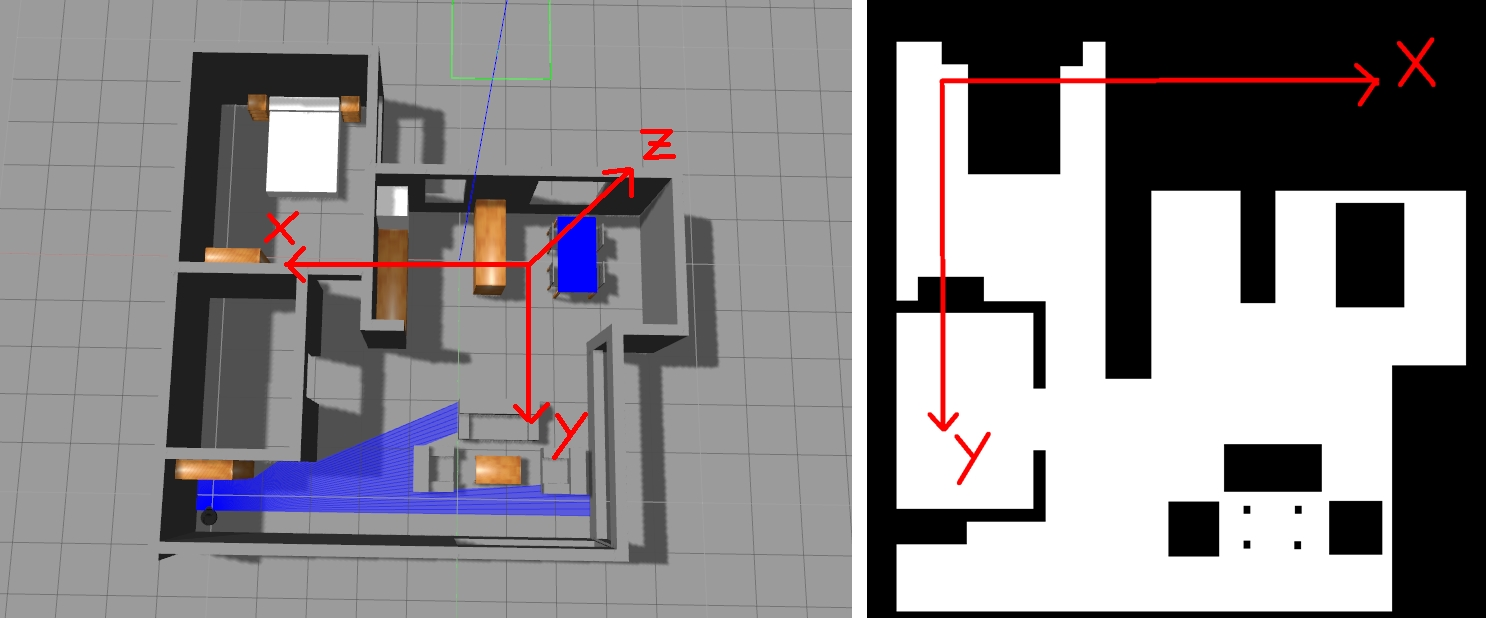
\includegraphics[width=1.0\textwidth]{figures/Vacuum/sistemaRef.jpg}
		\caption{Sistema de referencia de Gazebo y sistema de referencia del mapa}
		\label{fig.sistemaRef}
		\end{center}
\end{figure}


Para realizar la conversión de un sistema a otro hay que pasar de una coordenada (x, y, z) en Gazebo a una coordenada (x', y') en el mapa. Para ello se ha aplicado una rotación de \(\pi\) grados sobre el eje Y y también ha sido necesario añadir una traslación para conseguir tener el origen de coordenadas (0,0) de la imagen en la esquina superior izquierda. En concreto, se ha realizado una traslación de 0,6 en el eje X y de -1 en el eje Y. La siguiente matriz de rotación y traslación del eje Y~\ref{ec.matriz_roomba} es la matriz utilizada. El ángulo \(\alpha\) de la matriz será el ángulo de rotación en el eje Y; tx será la traslación en el eje X; ty será la traslación en el eje Y; y tz será la traslación en el eje Z. 

\begin{equation}
\label{ec.matriz_roomba}
\left[\begin{array}{cccc}
\cos(\alpha) & 0 & \sin(\alpha) & tx \\ 
0 & 1 & 0 & ty\\
-\sin(\alpha) & 0 & \cos(\alpha) & tz \\
0 & 0 & 0 & 1
\end{array}\right]
\end{equation}
\\


También es necesario multiplicar el resultado de aplicar la matriz por la escala, que indica el número de píxeles de la imagen que equivalen a un metro en el mundo de Gazebo. En este caso se ha establecido una escala de 50 píxeles por metro, por lo que la ecuación final~\ref{ec.ec_final} quedaría de la siguiente manera:

\begin{equation}
\label{ec.ec_final}
\left[\begin{array}{cc}
x' \\ 
y' \\
z' \\
1
\end{array}\right] = \left[\begin{array}{cccc}
\cos(\alpha) & 0 & \sin(\alpha) & tx \\ 
0 & 1 & 0 & ty\\
-\sin(\alpha) & 0 & \cos(\alpha) & tz \\
0 & 0 & 0 & 1
\end{array}\right]* \left[\begin{array}{cc}
x \\ 
y \\
z \\
1
\end{array}\right]*scale
\end{equation}


Gracias a esta transformación se puede pintar el triángulo, que representa a la aspiradora, aplicando la matriz de rotación y traslación a la coordenada de la posición de la aspiradora que se obtiene mediante el \textit{pose3d}. Esta coordenada será el centro del triángulo, que es isósceles para mostrar cuál es la orientación del robot que estará orientado hacia el vértice del triángulo de ángulo menor.\\

Para pintar las zonas azules por las que pasa la aspiradora es necesario guardar en un array los puntos que ocupa la aspiradora que se pintarán en cada iteración. 



Esta rotación también sirve para pintar en azul los puntos del mapa por donde ha pasado la aspiradora en cualquier momento. Se pintará un círculo en cada iteración dado que la aspiradora ocupa un determinado volumen. Los puntos por los que ha pasado la aspiradora se guardan en un array para saber por dónde ha pasado y pintarlos todos en cada iteración.\\

Por otro lado, a la derecha, hay un teleoperador bidimendional que permite mover el robot manualmente. La velocidad lineal se puede controlar moviendo el \textit{joystick} en el eje vertical y la velocidad angular se controla moviendo el \textit{joystick} en sentido horizontal.\\

En la parte inferior, aparecen dos botones. El botón situado bajo el mapa de la casa, permite tanto ejecutar como parar el código alojado en el archivo \textit{MyAlgorithm.py}. Con el botón que está debajo, se puede detener al robot si se está controlando manualmente con el teleoperador.\\


En la Figura~\ref{fig.vacuumGUI} se muestra el resultado de la interfaz gráfica que verá el usuario en todo momento y en ella, en la esquina superior izquierda, el logo de JdeRobot.

\begin{figure}[H]
  \begin{center}
    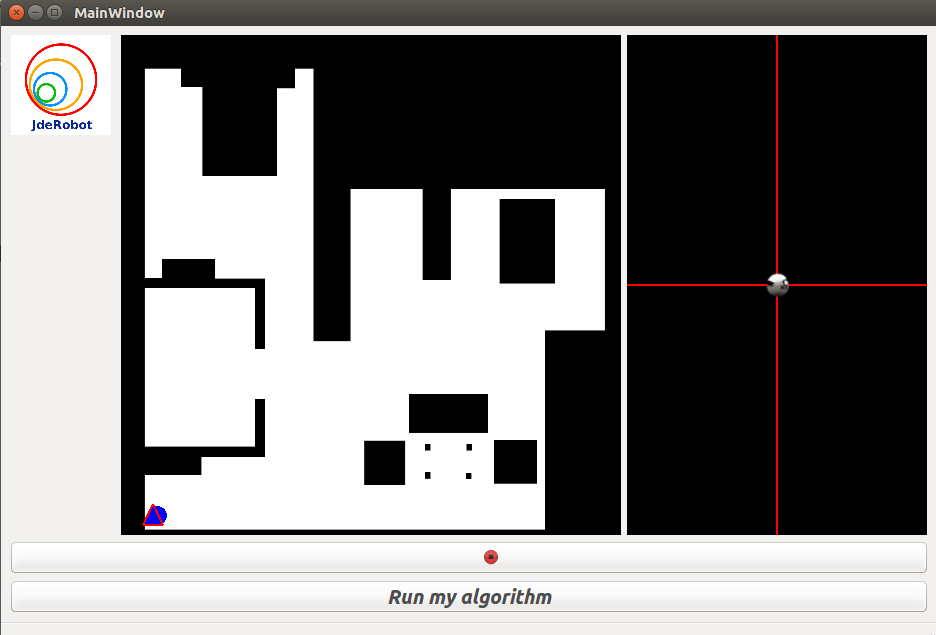
\includegraphics[width=1.0\textwidth]{figures/Vacuum/vacuumGUI.png}
		\caption{Interfaz gráfica}
		\label{fig.vacuumGUI}
		\end{center}
\end{figure}



\section{Solución de referencia} 
En esta práctica se plantea un problema de barrido de superficie en el que un robot aspirador tiene que ser capaz de recorrer la mayor parte posible del suelo de una casa haciendo uso de su capacidad de autolocalización y del mapa de dicha casa. La solución se ha programado en el fichero \textit{MyAlgorithm.py}, en el método \textit{``execute''}, que es el método principal de la solución. \\

La solución puede dividirse en dos partes principales: (a) planificación de la ruta; (b)Pilotaje del robot. 

\subsection{Planificación de la ruta}

Para calcular la ruta de la aspiradora, será necesario crear un algoritmo en zigzag. Para llevarlo a cabo, se creará una rejilla o malla de navegación sobre el mapa de la casa. Idealmente, el tamaño de las celdas que forman la malla serían del mismo tamaño que el robot, pero en esta solución es ligeramente inferior al tamaño de la aspiradora (17 x 17 píxeles), en concreto, miden 16 x 16 píxeles. Esto es debido a que las medidas de la celda deben ser un número par para poder realizar correctamente el cálculo y de esta manera, nos aseguramos de que no queden zonas sin barrer ya que si la celda ocupase más que la aspiradora quedarían zonas sin recorrer entre los trayectos del zigzag. \\

El mapa que la aspiradora utilizará tanto para comprobar el valor de las celdas como para ir marcando las zonas por las que ya ha pasado, será un mapa de la casa con los obstáculos dilatados (Figura~\ref{fig.obsDil}). Utilizando la operación morfológica de erosión conseguimos que la parte negra del mapa, es decir, los obstáculos, se amplíen ligeramente más que la mitad del tamaño de la aspiradora para asegurar que ésta no se choque con ningún obstáculo (ya que la aspiradora ocupa más que las celdas y tenemos que dar un margen de error para la navegación). En la Figura~\ref{fig.diff} aparece la diferencia entre el mapa original y el mapa con la dilatación de los obstáculos. 

\begin{figure}[H]
  \begin{center}
    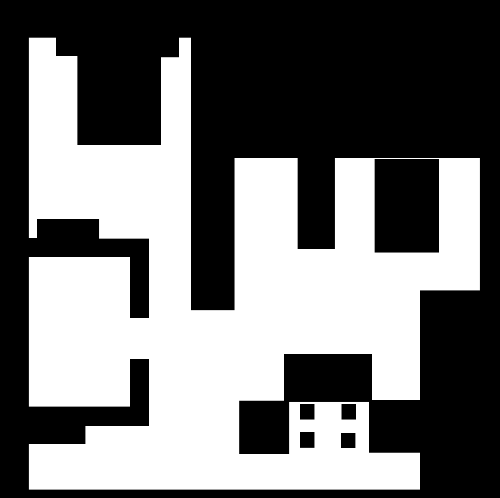
\includegraphics[width=0.7\textwidth]{figures/Vacuum/MapaErosionado.png}
		\caption{Mapa con los obstáculos dilatados}
		\label{fig.obsDil}
		\end{center}
\end{figure}

\begin{figure}[H]
  \begin{center}
    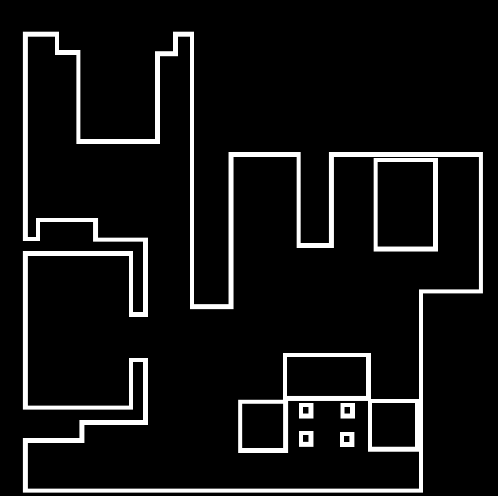
\includegraphics[width=0.7\textwidth]{figures/Vacuum/Diff.png}
		\caption{Diferencia entre el mapa original y el erosionado}
		\label{fig.diff}
		\end{center}
\end{figure}


En primer lugar calcularemos la celda en la que se encuentra la aspiradora a partir de su posición inicial. Para realizar la transformación de coordenadas de Gazebo a píxeles en el mapa, hemos creado la función \textit{``coord2pix''} que aplicará la ecuación~\ref{ec.ec_final}, y para realizar la transformación inversa, es decir, de píxeles a coordenadas, hemos creado la función \textit{``pix2coord''} que aplicará la matriz de rotación y traslación inversa. Una vez ubicada la aspiradora en el mapa y creada la primera celda, se irán calculando las celdas contiguas a ésta mediante la función \textit{``calculateNeigh''} que calculará las celdas vecinas: Norte, Este, Oeste y Sur. En la Figura~\ref{fig.neighZoom} se puede ver como queda la disposición de las celdas en el mapa, siendo C la celda donde se encuentra la aspiradora, N la celda Norte, E la Este, O la Oeste y S la Sur.

\begin{figure}[H]
  \begin{center}
    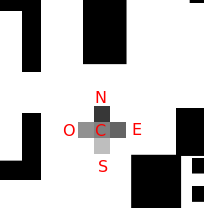
\includegraphics[width=0.4\textwidth]{figures/Vacuum/neighZoom.png}
		\caption{Ejemplo de vecindad de las celdas}
		\label{fig.neighZoom}
		\end{center}
\end{figure}

Las celdas podrán tener tres valores:

\begin{itemize}
\item Obstáculo: Al menos uno de los píxeles que forman la celda es negro, es decir forma parte de un obstáculo de la casa.
\item Obstáculo virtual: La aspiradora ya ha pasado por esta casilla y la marcará de color gris en el mapa. 
\item Libre: Todos los píxeles de la celda son blancos, es decir, no contienen ningún tipo de obstáculo (ni normal ni virtual).
\end{itemize}

Para saber el valor que tiene cada casilla hemos creado la función \textit{``checkCell''} que comprobará todos los píxeles de la celda e indicará cuál es su valor correspondiente.\\

Mediante la función \textit{``zigzag''} calcularemos la siguiente celda a la que tiene que moverse la aspiradora llevando a cabo la lógica del zigzag, y hasta que no haya conseguido llegar a ese punto, no se calculará la siguiente casilla. Este algoritmo consistirá en que la aspiradora avanzará hacia adelante siempre y cuando la casilla Norte esté libre. Si encuentra un obstáculo (normal o virtual), la aspiradora se moverá hacia su derecha, es decir, hacia la celda Este y después avanzará hacia el sur hasta que vuelva a encontrar otro obstáculo, en cuyo caso, volverá a desplazarse a la celda Este y después hacia el norte y así sucesivamente. En el caso de que la celda Este estuviera ocupada, la aspiradora avanzará hacia la celda Oeste. En la Figura ~\ref{fig.ejemplo} se muestra un ejemplo sencillo de como quedaría idealmente el algoritmo donde la aspiradora inicialmente estaría en la celda con el punto azul y terminaría en la del punto verde.

\begin{figure}[H]
  \begin{center}
    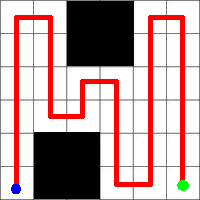
\includegraphics[width=0.5\textwidth]{figures/Vacuum/cuadriculaEj.png}
		\caption{Ejemplo de zigzag}
		\label{fig.ejemplo}
		\end{center}
\end{figure}

Seguirá realizando estos pasos hasta que llegue a una casilla en la que todas las celdas adyacentes sean obstáculos tanto normales como virtuales. A esta situación la denominaremos punto crítico.

\subsubsection{Ruta de retorno}
Si la aspiradora llega a un punto crítico y no puede avanzar más porque está rodeada de obstáculos, deberá ser capaz de calcular una ruta para retornar a otra zona del mapa y continuar con un nuevo zigzag. La función creada \textit{``isCriticalPoint''} comprobará, cada vez que la aspiradora llegue a una celda nueva, si se trata o no de un punto crítico chequeando todos los vecinos de dicha celda.\\

El algoritmo de retorno, se calculará a partir de las celdas que ya ha recorrido la aspiradora. De esta manera, aseguramos que todas las celdas están libres de obstáculos. Según vaya avanzando la aspiradora, guardará todas las celdas por las que ha ido pasando mediante la función \textit{``savePath''}. Además, guardará las celdas que posiblemente puedan consderarse puntos de retorno. Un punto de retorno lo definimos como aquella celda que tiene uno o más vecinos libres. Para ello, hemos creado la función \textit{``isReturnPoint''} que indica si la celda correspondiente es un punto de retorno o no.\\

En el momento en que la aspiradora llega a un punto crítico, deberá comprobar todos los puntos de retorno que ha ido guardando ya que es posible que a lo largo del trayecto, la aspiradora haya recorrido las celdas vecinas de algunos de estos puntos. Para ello hemos creado la función \textit{``checkReturnPoints''} que comprobará si los puntos de retorno guardados tienen o no celdas vecinas libres y en cuyo caso se eliminarán. \\

Para decidir a que punto de retorno dirigirse, nos basaremos en elegir el punto más cercano a la posición de la aspiradora. Hemos creado la función \textit{checkMinDist} que mide la distancia euclídea (ecuación ~\ref{ec.distEuclidea}) entre la aspiradora y todos los puntos de retorno que haya y elige el punto más cercano.

\begin{equation}
\label{ec.distEuclidea}
d_{E}(P_{1}, P_{2}) = \sqrt{(x_{2} - x_{1})^{2} + (y_{2} - y_{1})^{2}}
\end{equation}

Una vez elegido el punto al que retornar, la aspiradora mediante la función \textit{goToReturnPoint} se dirijirá a dicho punto. Esta función llevará a cabo el cálculo de las distintas celdas a las que la aspiradora tiene que desplazarse y de verificar si la aspiradora ha llegado a ellas. Para calcular la trayectoria de retorno hemos creado la función \textit{searchReturnPath} que se encarga de comprobar si existe visibilidad entre la celda de retorno y la celda donde se encuentra la aspiradora. Dos puntos tienen visibilidad entre sí, si los puntos de la recta que los une están libres de obstáculos. Si existe visibilidad directa entre el punto de retorno y la posición de la aspiradora, la trayectoria de retorno consistirá solo en estas dos celdas ya que habría vía libre de obstáculos entre ambos. En el caso contrario, sería necesario encontrar celdas intermedias. Estas celdas se buscarían en el camino que ha seguido la aspiradora ya que son celdas sin obstáculos. Cuando se encontrase una celda que tenga visibilidad con la aspiradora también se comprobaría si tiene visibilidad con la celda de retorno. Si hay visibilidad con ambas solo sería necesario una celda intermedia, pero si no, se volvería buscar la visibilidad entre las celdas del camino y la celda intermedia y así sucesivamente hasta conseguir encontrar la ruta con celdas que tengan visibilidad entre sí.\\

Para calcular la visibilidad entre dos celdas hemos creado la función \textit{visibility}. Esta función comprobará si la recta que une a las dos celdas está libre de obstáculos. Como es imposible comprobar todos los puntos que contienen a la recta, se comprobarán los que hay cada 10 cm. Dichos puntos se calcularán mediante la ecuación ~\ref{ec.recta} donde A y B son los puntos de inicio y final la recta, P es el punto intermedio y S es el paso, es decir, la distancia entre A y P. Esta ecuación la llevará a cabo la función \textit{pointOfLine}. Para constatar si alguno de los puntos de la recta forma parte de un obstáculo, hemos creado la función \textit{isObstacle}, que comprobará si el punto corresponde a un píxel blanco o negro en el mapa.

\begin{equation}
\label{ec.recta}
P = A + S(B - A)
\end{equation}


Para comprobar la visibilidad entre dos celdas, utilizamos un mapa de la casa con los obstáculos dilatados el tamaño de la aspiradora para evitar que ésta se choque con las esquinas de los obstáculos (Figura ~\ref{fig.mapaVis}).

\begin{figure}[H]
  \begin{center}
    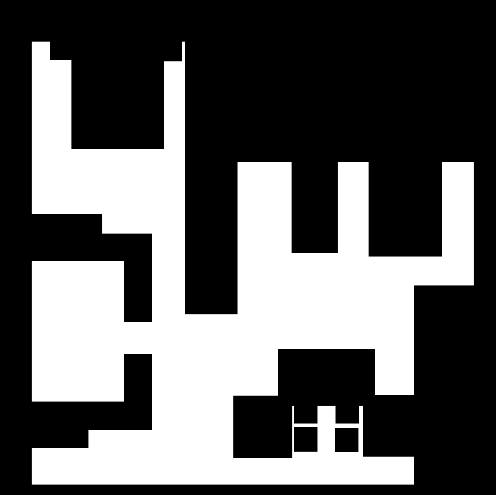
\includegraphics[width=0.7\textwidth]{figures/Vacuum/mapaVis.png}
		\caption{Mapa usado para la visibilidad entre dos celdas}
		\label{fig.mapaVis}
		\end{center}
\end{figure}

\begin{figure}[H]
  \begin{center}
    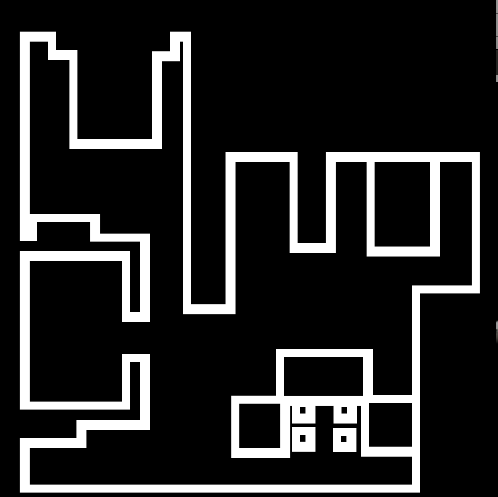
\includegraphics[width=0.7\textwidth]{figures/Vacuum/diffVis.png}
		\caption{Diferencia entre el mapa original y el de la visibilidad}
		\label{fig.diffVis}
		\end{center}
\end{figure}


En el mapa de la izquierda de la Figura  ~\ref{fig.rutaRet} se puede ver un ejemplo de como el algoritmo va buscando las celdas intermedias que forman el camino de retorno ya que que no existe visibilidad entre las celdas de retorno y la que contiene a la aspiradora. En el mapa de la derecha se muestra en color gris las celdas por las que la aspiradora ya ha pasado, en azul la celda donde se encuentra la aspiradora, en verde la celda de retorno, en amarillo la celda intermedia y en rojo la trayectoria calculada.\\

\begin{figure}[H]
  \begin{center}
    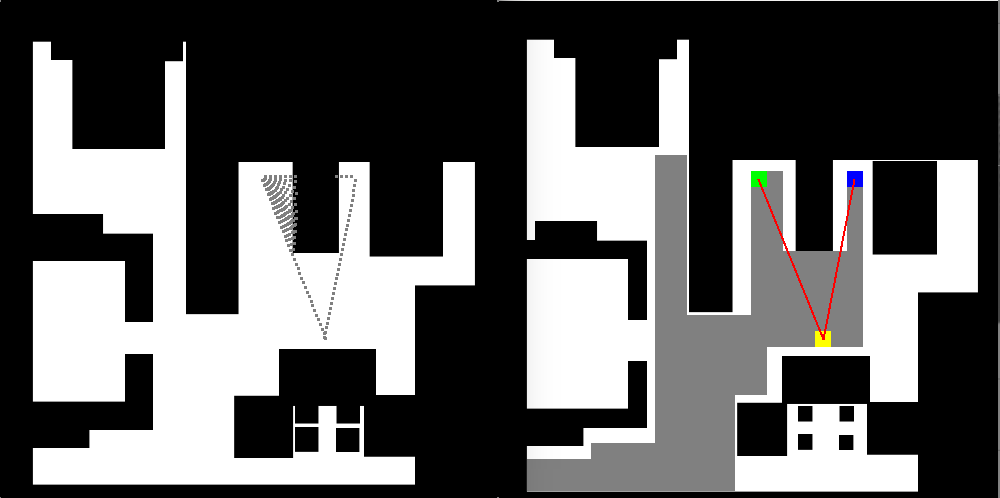
\includegraphics[width=1.0\textwidth]{figures/Vacuum/visibilidadEntreDosPuntos.png}
		\caption{Cálculo de la ruta de retorno}
		\label{fig.rutaRet}
		\end{center}
\end{figure}

El algoritmo de barrido finalizará cuando la aspiradora esté en un punto crítico y no queden puntos a los que retornar.


\subsection{Pilotaje del robot}

Una vez calculada la celda a la cual la aspiradora se tiene que dirigir, es necesario crear un algoritmo que se encargue del movimiento del robot. Para ello hemos creado la función \textit{goToCell} que recibirá la celda destino y calculará la desviación (con la función \textit{calculateDesv)} de dicha celda respecto de la aspiradora. Para realizar este cálculo, necesitamos convertir las coordenadas absolutas de la celda a coordenadas relativas al robot mediante la función \textit{abs2rel}. Esta función aplicará una rotación a las coordenadas según la orientación de la aspiradora.\\

Tanto la velocidad de giro como la velocidad lineal de la aspiradora se determinarán según la desviación que haya entre la celda y el robot. Si la desviación es elevada, estableceremos una velocidad de giro alta y pararemos la aspiradora para que se alinee rápidamente con la celda y no avance desviada. Según vaya disminuyendo la desviación, aumentaremos de manera gradual la velocidad lineal y reduciremos la de giro hasta conseguir que la aspiradora esté alineada con la celda. Dichos cambios de velocidad se llevarán a cabo mediante las funciones \textit{controlDrive} y \textit{controlDesv}. \\


En el caso de que la aspiradora tenga que recorrer varias celdas consecutivas (en la dirección norte o sur), aumentaremos la velocidad lineal de manera proporcional a las casillas libres que tenga delante, disminuyendo así, el tiempo que tarda la aspiradora en recorrer la casa entera. Para ello, hemos creado la función \textit{setV}, que calcula las cuatro celdas siguientes en la dirección correspondiente y según las que haya libres, aumentará o reducirá la velocidad lineal de la aspiradora. En el caso de estar realizando una ruta de retorno, la velocidad se ajustará según la distancia entre la celda y la aspiradora, yendo más rápido cuanto más lejos se encuentren entre sí.\\

La función \textit{driving} irá comprobando si la aspiradora ha llegado a la celda destino. Para realizar esta comprobación hemos creado la función \textit{checkArriveCell} que dará por conseguida la celda, si la aspiradora se encuentra en el centro de dicha celda. Es necesario establecer un margen de error ya que la aspiradora se encuentra en movimiento. Este umbral será mayor cuando la aspiradora tenga que recorrer varias celdas consecutivas (en la dirección norte o sur). En el caso en el que la aspiradora tenga que girar o si en la siguiente celda hay un obstáculo (normal o virtual), el umbral será menor para ajustar lo máximo posible la ruta en forma de zigzag. 



\section{Evaluador automático} 
Para esta práctica se ha creado un evaluador automático que, basándose en diferentes parámetros, brindará una calificación final a la solución realizada por el alumno. Al igual que en el componente académico, también se ha utilizado la herramienta PyQt5 para su creación. El evaluador muestra una interfaz gráfica en la que aparecen los parámetros que medirá para el cálculo de la nota final.\\

En la esquina superior izquierda aparece una barra de progreso que se irá rellenando de color rojo proporcionalmente a la superficie recorrida por el robot. Para calcular el porcentaje recorrido, se tiene en cuenta que el 100 \% de la superficie son todos los píxeles blancos del mapa. Según la aspiradora vaya moviéndose por la casa, se irá guardando el número de píxeles correspondientes a las zonas ocupadas y se realizará el cálculo del porcentaje de la casa al que correspondan. Esta información también aparece de manera numérica encima de la barra de progreso.\\

Al igual que en la interfaz gráfica del componente académico, a la izquierda, se muestra el mapa de la casa y en él, las zonas por las que va pasando la aspiradora pintadas en azul. Igualmente, ha sido necesario utilizar la ecuación ~\ref{ec.ec_final} y aplicar una rotación de \(\pi\) grados sobre el eje Y, una traslación de 0,6 en el eje X y de -1 en el eje Y, y usar la misma escala. En este caso, no se muestra la orientación de la aspiradora.\\

En la parte derecha, aparece un reloj digital que indica el número de segundos restantes hasta la finalización de la prueba. Al comenzar la prueba aparecerán 900 segundos (15 minutos). Se ha elegido este tiempo ya que se ha considerado que es el más idóneo para evaluar la práctica. Si se escogiera un tiempo mayor la evaluación de la práctica sería muy lenta y si se optase por un tiempo menor, no habría datos suficientes para calcular la nota. \\

Debajo de este reloj digital, se muestra un reloj analógico que va avanzando cada segundo que pasa. \\


Por último, una vez que el tiempo de ejecución finaliza, a la derecha del reloj digital aparecerá un mensaje con la nota que ha obtenido el alumno. La calificación obtenida será directamente proporcional al porcentaje de superficie recorrida. Si pasados los 15 minutos, el alumno ha conseguido que la aspiradora recorra el 35 \% de la superficie o más, obtendrá la máxima nota, un 10. Si por el contrario recorre menos superficie se realizará una regla de tres sabiendo que el 35 \% es un 10.\\

Este evaluador se ha desarrollado en el archivo llamado \textit{``referee.py''}. En la Figura~\ref{fig.referee} se muestra el resultado de la interfaz gráfica que se mostrará después de un tiempo ejecutando la solución creada y en ella, en la parte inferior, el logo de JdeRobot después de un tiempo ejecutando la solución creada.

\begin{figure}[H]
  \begin{center}
    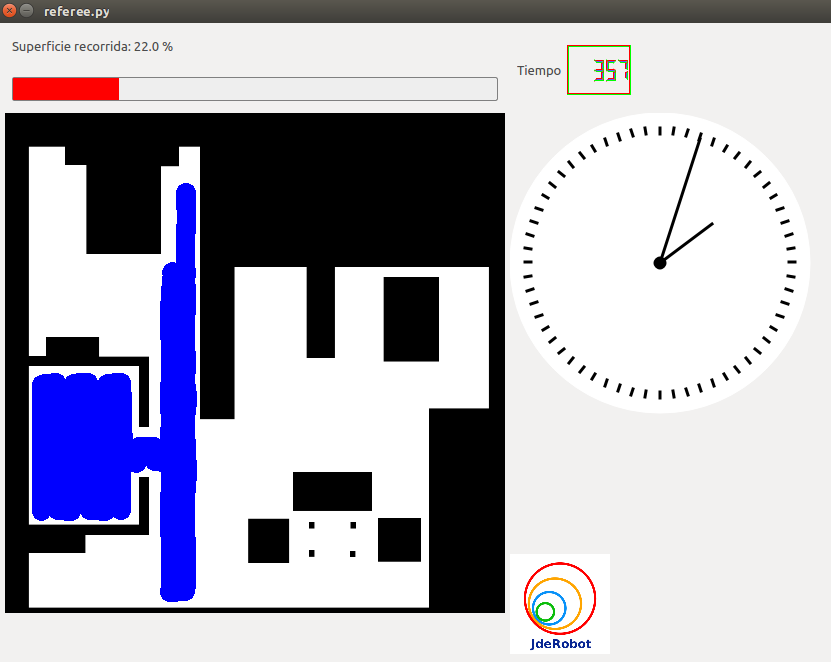
\includegraphics[width=1.0\textwidth]{figures/Vacuum/refereeTiempo.png}
		\caption{Evaluador automático}
		\label{fig.referee}
		\end{center}
\end{figure}



\section{Experimentación} 

\subsection{Ejecución típica}
Para ejecutar esta práctica, es necesario abrir tres terminales y ejecutar los siguientes comandos:

\begin{enumerate}[1.]
\item Lanzar el simulador Gazebo:
	\begin{lstlisting}[frame=single]
		gazebo vacuum.world
	\end{lstlisting} 
	\begin{enumerate}[1b.]
	\item Se puede arrancar solo el simulador sin la interfaz gráfica:
		\begin{lstlisting}[frame=single]
		 	gzserver vacuum.world
		\end{lstlisting}
	\end{enumerate}
\end{enumerate}

\begin{enumerate}[2.]
\item	Ejecutar la práctica y lanzar la interfaz gráfica (\acrshort{gui}): 
	\begin{lstlisting}[frame=single]
		python2 vacuum.py -- --Ice.Config=vacuum.cfg
	\end{lstlisting} 
\end{enumerate}

\begin{enumerate}[3.]
\item	Ejecutar el evaluador automático: 
	\begin{lstlisting}[frame=single]
		python2 referee.py -- --Ice.Config=vacuum.cfg
  	\end{lstlisting} 
\end{enumerate}

En la siguiente imagen (Figura ~\ref{fig.ejTipica}) se puede observar el resultado de una ejecución típica de 15 minutos.

\begin{figure}[H]
  \begin{center}
    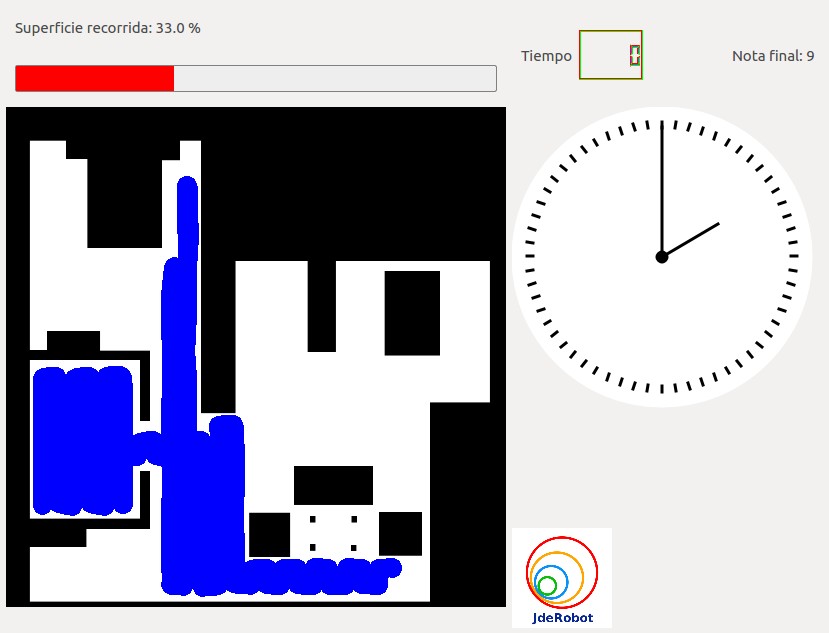
\includegraphics[width=1.0\textwidth]{figures/Vacuum/ejecucionTipicaRefereeSala.png}
		\caption{Ejecución típica}
		\label{fig.ejTipica}
		\end{center}
\end{figure}




\subsection{Experimentos de larga duración}

Con una ejecución típica no se puede apreciar si realmente el algoritmo programado recorre la casa entera o no, por lo que se ha realizado una ejecución de larga duración para que de tiempo a llevar a cabo todo el algoritmo y que el robot recorra la casa entera.\\ 

En la siguiente imagen (Figura ~\ref{fig.sala}) se puede ver cómo con el algoritmo programado la aspiradora es capaz de recorrer la mayor parte de la superficie disponible, en concreto, el 74\%.

\begin{figure}[H]
  \begin{center}
    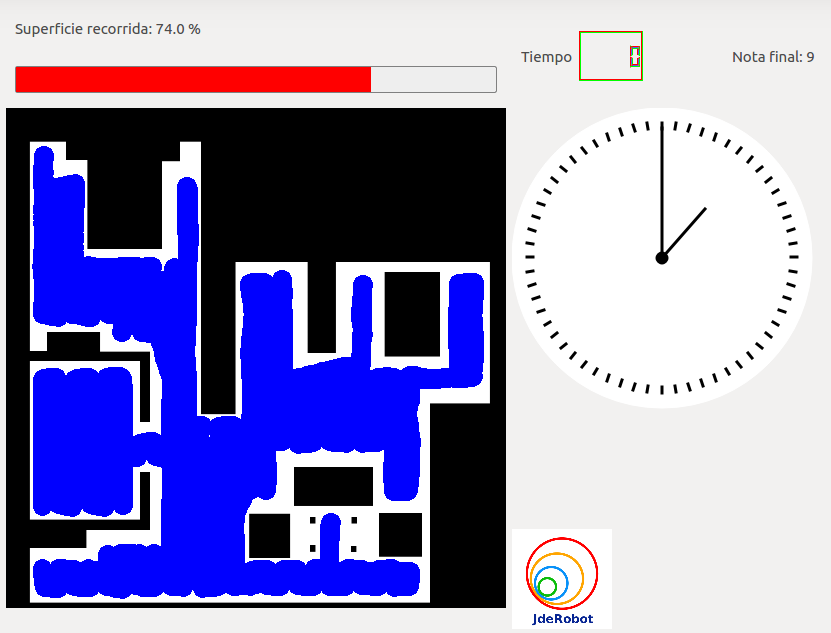
\includegraphics[width=1.0\textwidth]{figures/Vacuum/refereeSala.png}
		\caption{Ejecución de larga duración}
		\label{fig.sala}
		\end{center}
\end{figure}

La ejecución completa del algoritmo se puede ver en este vídeo \footnote{\url{https://www.youtube.com/watch?v=sUT5ru4Ew_E
}}.

\subsubsection{Inicio en distintos puntos de la casa}

La posición inicial del robot influirá en la cantidad de superficie recorrida, en la nota obtenida y en el tiempo que tarda en ejecutar completamente el algoritmo programado. Esto es debido a que la rejilla de navegación se va creando según las coordenadas iniciales del robot por lo que si por ejemplo, empieza más cerca de las paredes, puede que las celdas de la rejilla se ajusten más o menos a los obstáculos y sea capaz de recorrer más superficie. También influye en el tiempo porque puede que sea necesario hacer más rutas de retorno y esto aumentará el tiempo que tarda en recorrer la casa entera ya que pasará varias veces por zonas ya barridas.\\

Se han realizado varios experimentos cambiando la posición de inicio de la aspiradora. En la Tabla~\ref{table:resultados} se puede observar cómo la posición de inicio afecta a la superficie recorrida y al tiempo de ejecución necesario para barrer la casa entera.

\begin{table}[h!]
\centering
\caption{Resultados con distintas posiciones iniciales}
\begin{tabular}{|c|c|c|c|}
\hline
\textbf{Posición inicial}  & \textbf{Superficie recorrida} & \textbf{Tiempo de ejecución}  & \textbf{Nº rutas de retorno} \\ 
\hline
Sala (5.04, 3.80)    & 74 \%                        & 48 min 01 seg                         & 15\\ 
\hline
Dormitorio (5.04, 0.00)         & 75 \%                        & 47 min 07 seg    						& 15\\ 
\hline
Salón (-2.35, 5.44)          & 75 \%                        & 51 min 10 seg    						& 16\\ 
\hline
Comedor (-3.50, 1.45)      & 69 \%                        & 42 min 13 seg    						& 14\\ 
\hline
\end{tabular}

\label{table:resultados}
\end{table}

En la Figura ~\ref{fig.posInicio} aparecen marcadas las zonas de inicio seleccionadas. En verde aparece la posición denominada Sala, en rosa Dormitorio, en rojo Salón y en azul Comedor.

\begin{figure}[H]
  \begin{center}
    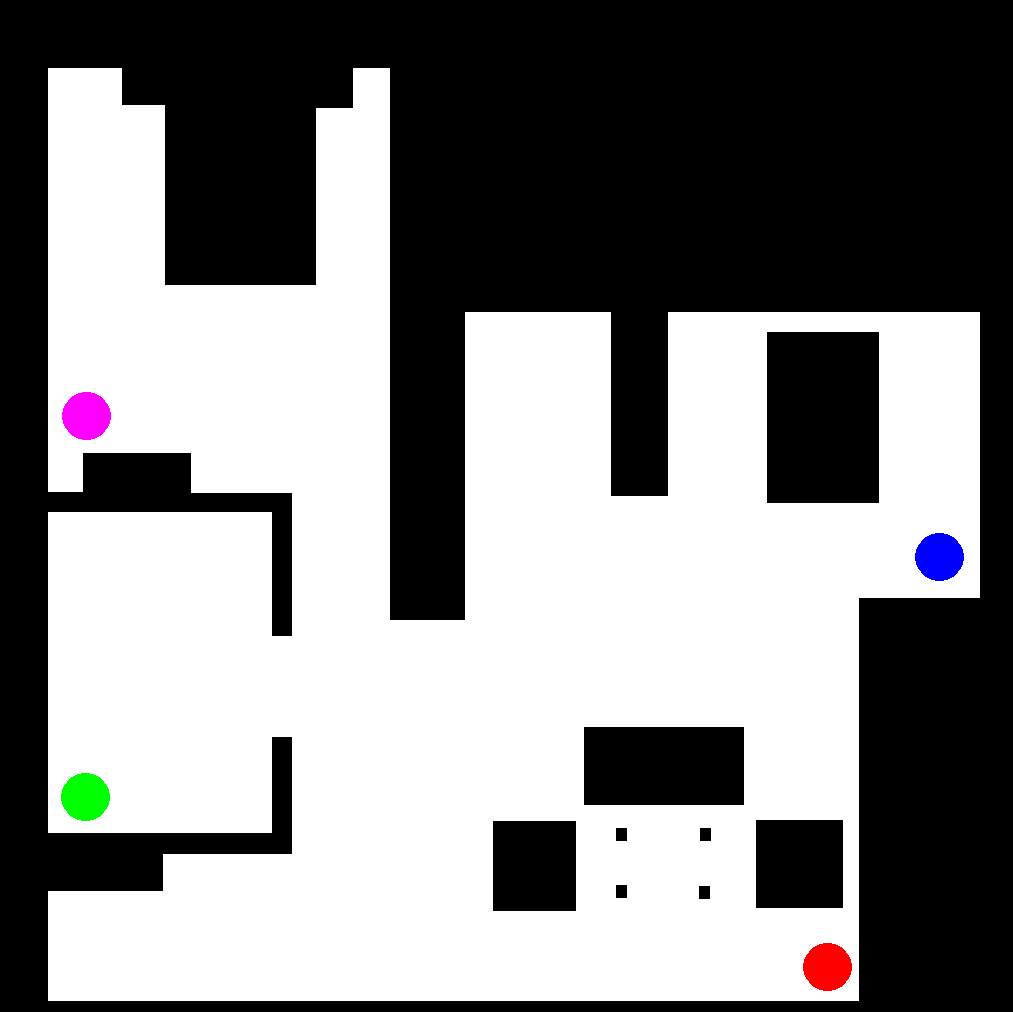
\includegraphics[width=0.7\textwidth]{figures/Vacuum/mapaPosInicio.png}
		\caption{Posiciones de inicio}
		\label{fig.posInicio}
		\end{center}
\end{figure}


A continuación se muestran los resultados obtenidos con la ejecución del algoritmo en las distintas posiciones marcadas anteriormente. 

\begin{figure}[H]
  \begin{center}
    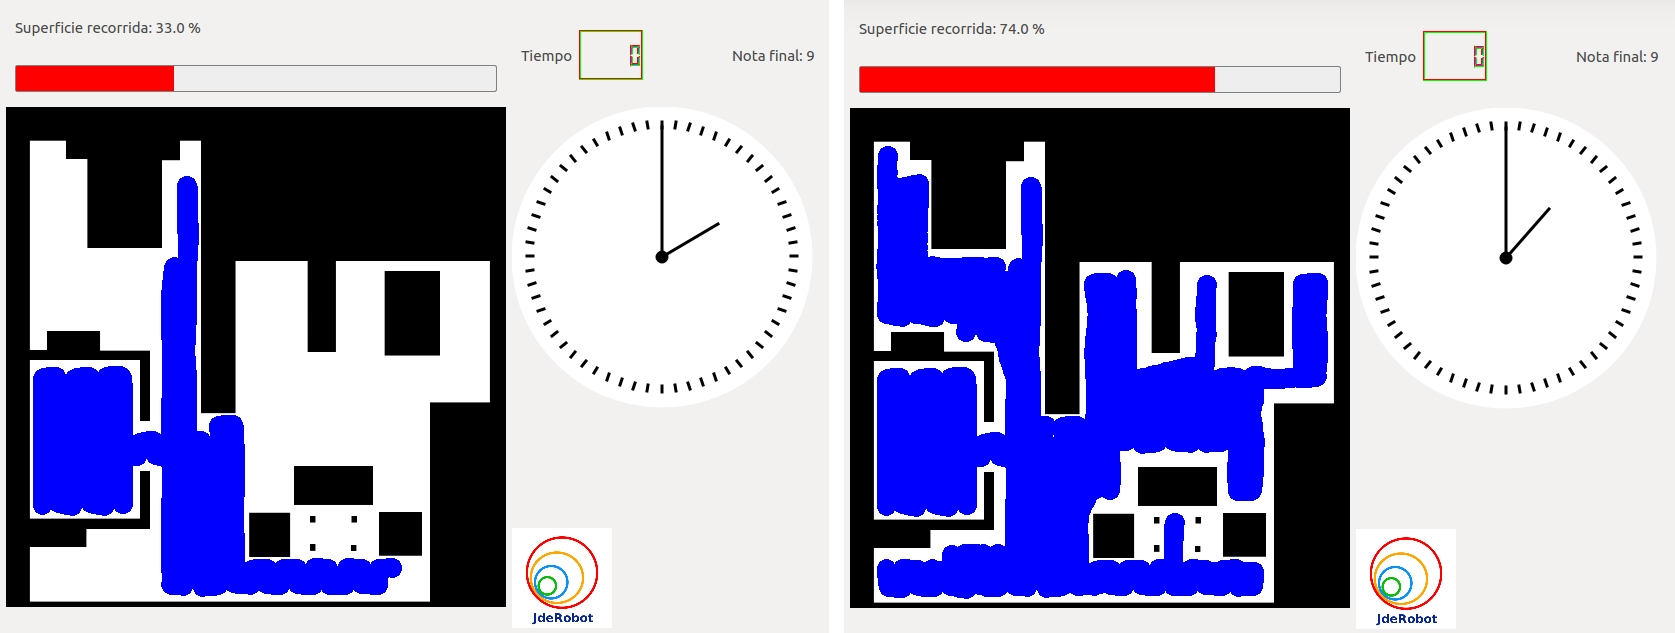
\includegraphics[width=1.0\textwidth]{figures/Vacuum/ejecucionSala.jpg}
		\caption{Ejecución típica y de larga duración en la posición inicial Sala}
		\label{fig.ejecucionSala}
		\end{center}
\end{figure}

\begin{figure}[H]
  \begin{center}
    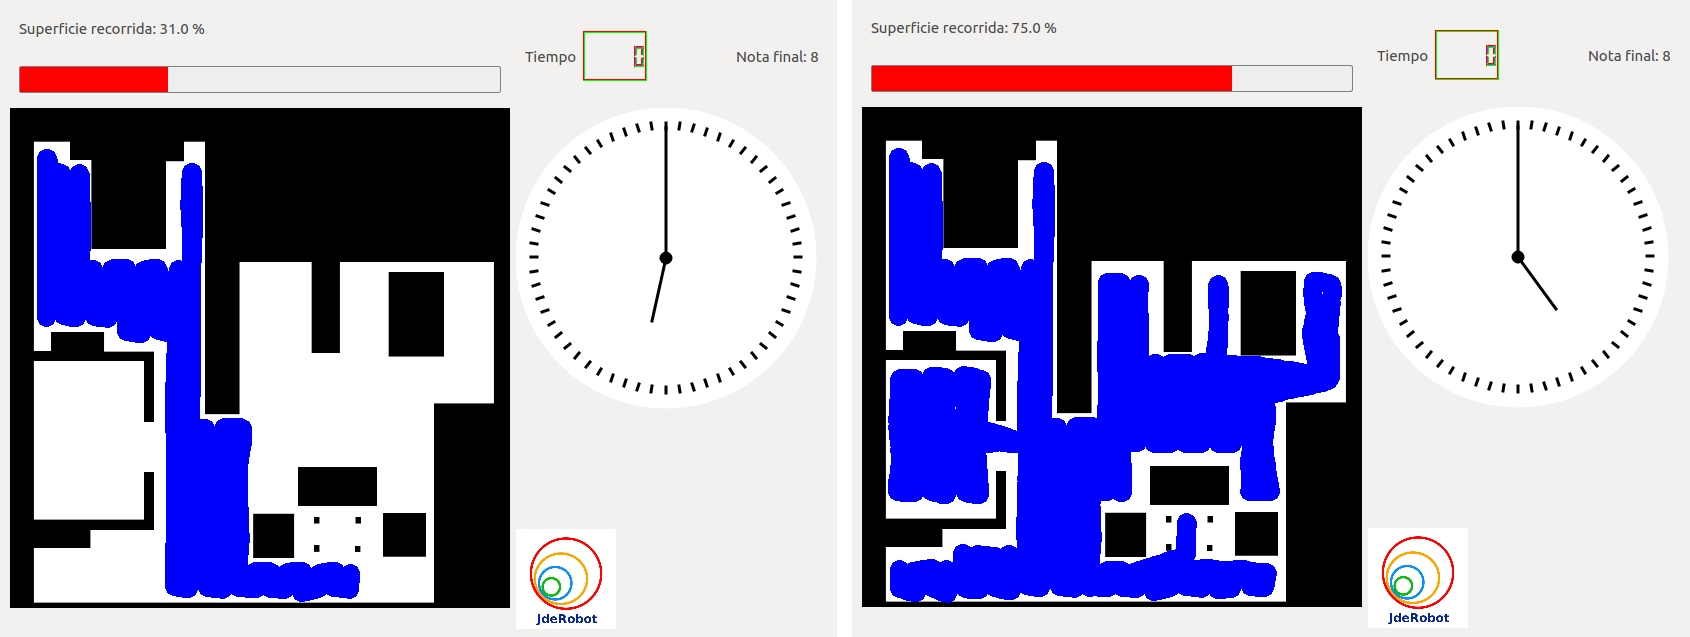
\includegraphics[width=1.0\textwidth]{figures/Vacuum/ejecucionHabitacion.jpg}
		\caption{Ejecución típica y de larga duración en la posición inicial Dormitorio}
		\label{fig.ejecucionDormitorio}
		\end{center}
\end{figure}

\begin{figure}[H]
  \begin{center}
    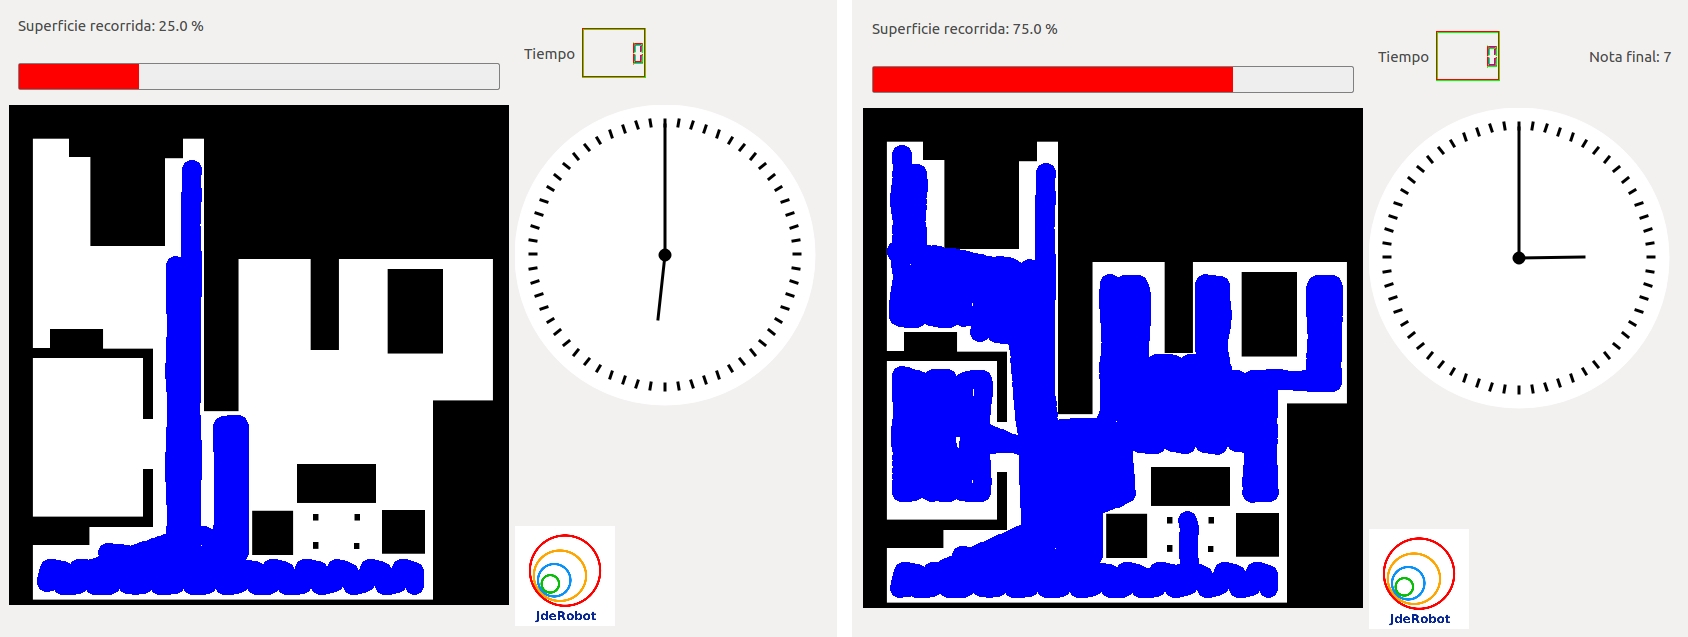
\includegraphics[width=1.0\textwidth]{figures/Vacuum/ejecucionSalon.jpg}
		\caption{Ejecución típica y de larga duración en la posición inicial Salon}
		\label{fig.ejecucionSalon}
		\end{center}
\end{figure}

\begin{figure}[H]
  \begin{center}
    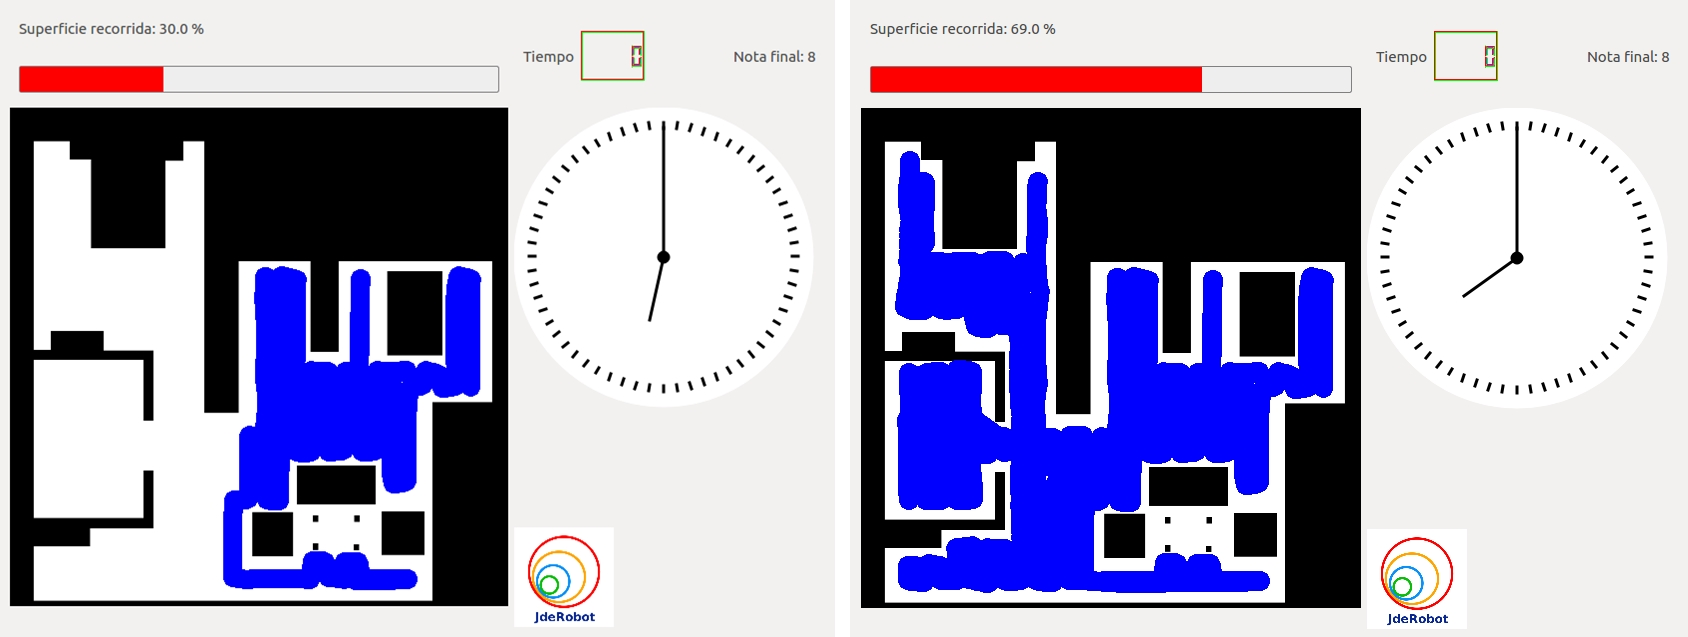
\includegraphics[width=1.0\textwidth]{figures/Vacuum/ejecucionComedor.jpg}
		\caption{Ejecución típica y de larga duración en la posición inicial Comedor}
		\label{fig.ejecucionComedor}
		\end{center}
\end{figure}
